% Q1: Faraday's Law — Circular coil of N turns in sinusoidal B field
\documentclass[border=10pt]{standalone}
\usepackage{tikz}
\usepackage{amsmath}
\renewcommand{\familydefault}{\sfdefault}

\begin{document}
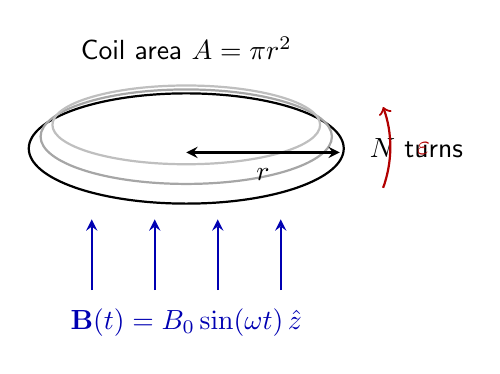
\begin{tikzpicture}[
    line width=0.8pt,
    every node/.style={font=\sffamily}
]

% Coil (represented as an ellipse — top-down view)
\draw[thick] (0,0) ellipse (2cm and 0.7cm);
% Second winding to suggest N turns
\draw[thick, gray!70] (0,0.15) ellipse (1.85cm and 0.6cm);
% Third winding
\draw[thick, gray!50] (0,0.30) ellipse (1.70cm and 0.5cm);

% N turns label
\node[right] at (2.2,0) {$N$ turns};

% Radius arrow
\draw[<->, >=stealth, thick] (0,-0.05) -- (1.95,-0.05)
    node[midway, below, yshift=-2pt] {$r$};

% B field arrows (upward, through coil)
\foreach \x in {-1.2, -0.4, 0.4, 1.2} {
    \draw[->, >=stealth, thick, blue!70!black] (\x, -1.8) -- (\x, -0.9);
}

% B field label
\node[blue!70!black, below] at (0, -1.9) {$\mathbf{B}(t) = B_0 \sin(\omega t)\,\hat{z}$};

% Axis label
\node[above] at (0, 1.0) {Coil area $A = \pi r^2$};

% EMF label with polarity
\draw[thick, red!70!black, ->] (2.5, -0.5) arc[start angle=-20, end angle=20, radius=1.5cm];
\node[red!70!black, right] at (2.8, 0) {$\varepsilon$};

\end{tikzpicture}
\end{document}
